\documentclass{article}
\usepackage[margin=1.2in]{geometry}
\usepackage[utf8]{inputenc}
\usepackage[english]{babel}
\usepackage{mathtools}
\usepackage[]{amsthm} %lets us use \begin{proof}
\usepackage[]{amssymb} %gives us the character \varnothing
\usepackage{algorithm}
\usepackage{algorithmic}


\title{Homework 1}
\author{Eric Geil}
\date\today
%This information doesn't actually show up on your document unless you use the maketitle command below
\begin{document}
\maketitle %This command prints the title based on information entered above

%Section and subsection automatically number unless you put the asterisk next to them.
\section{}
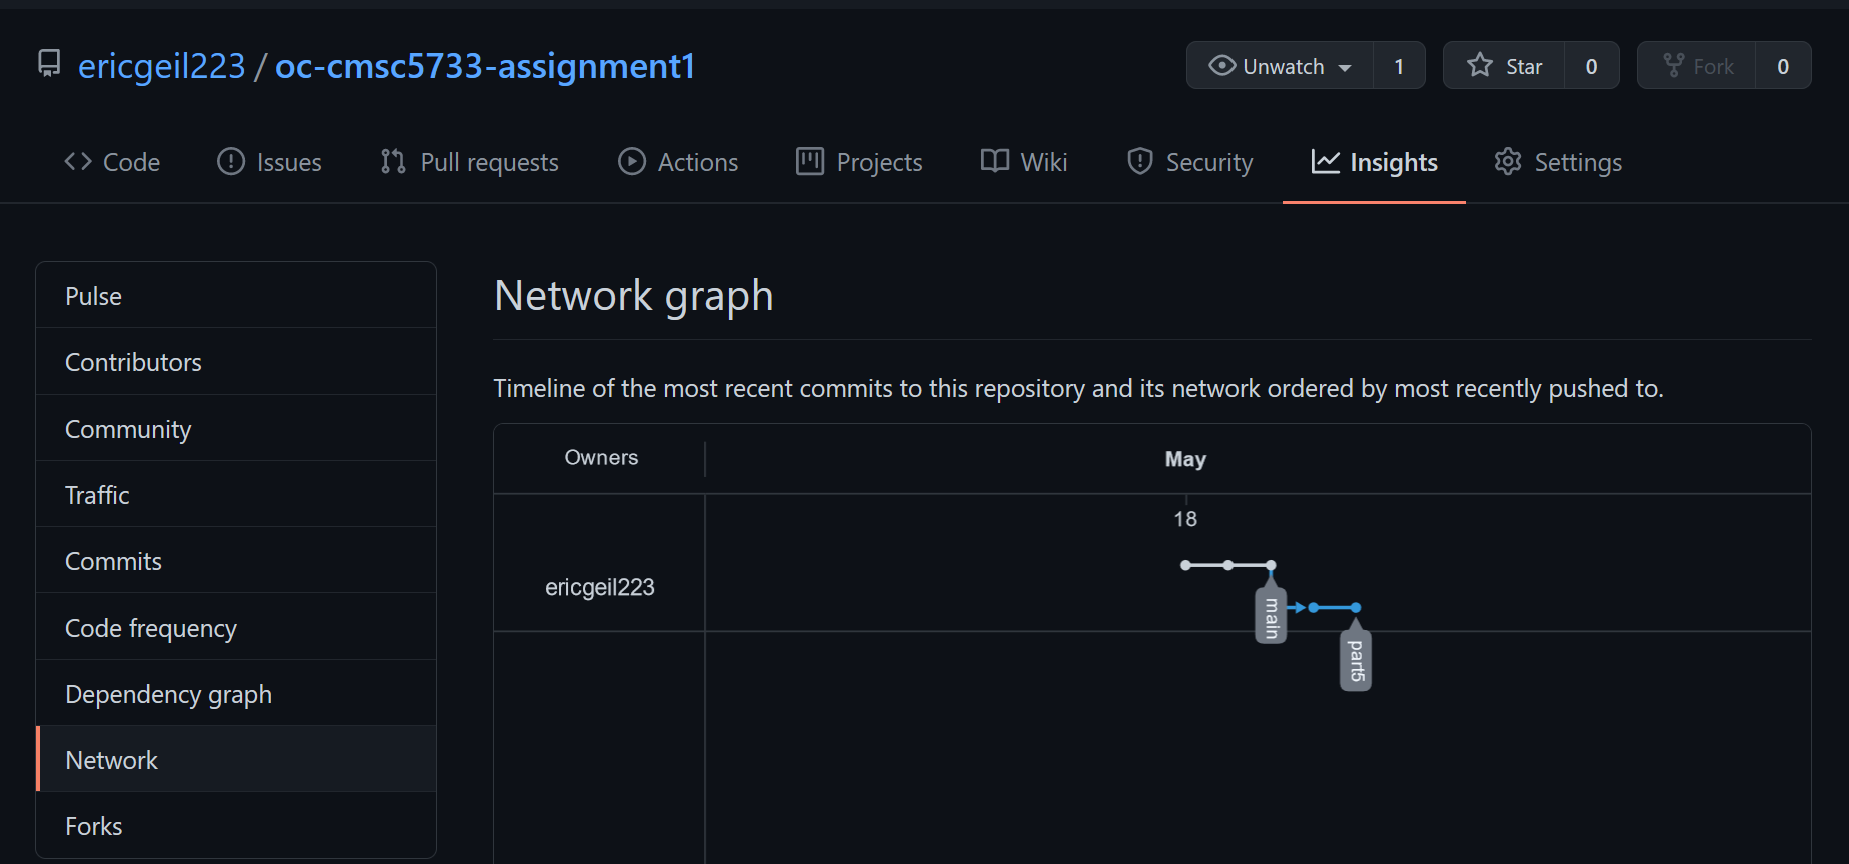
\includegraphics[width=1.0\textwidth]{2.png}
\section{}
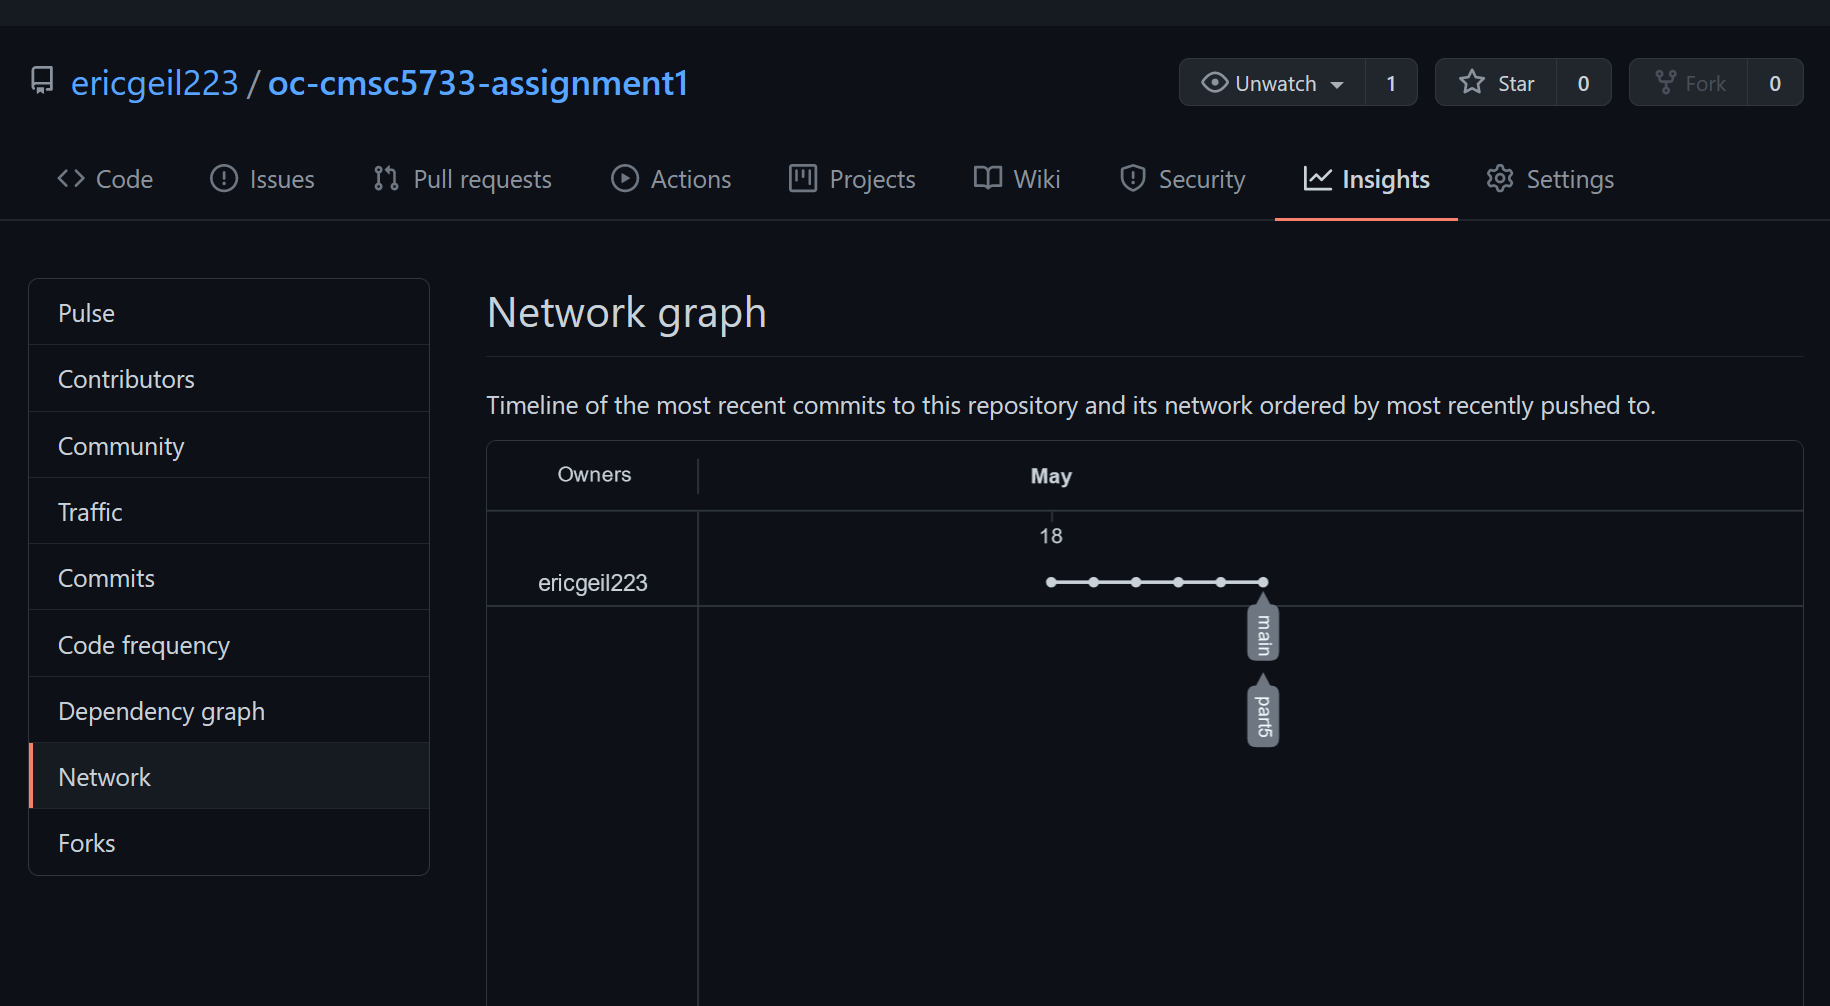
\includegraphics[width=1.0\textwidth]{3.png}
\section{}
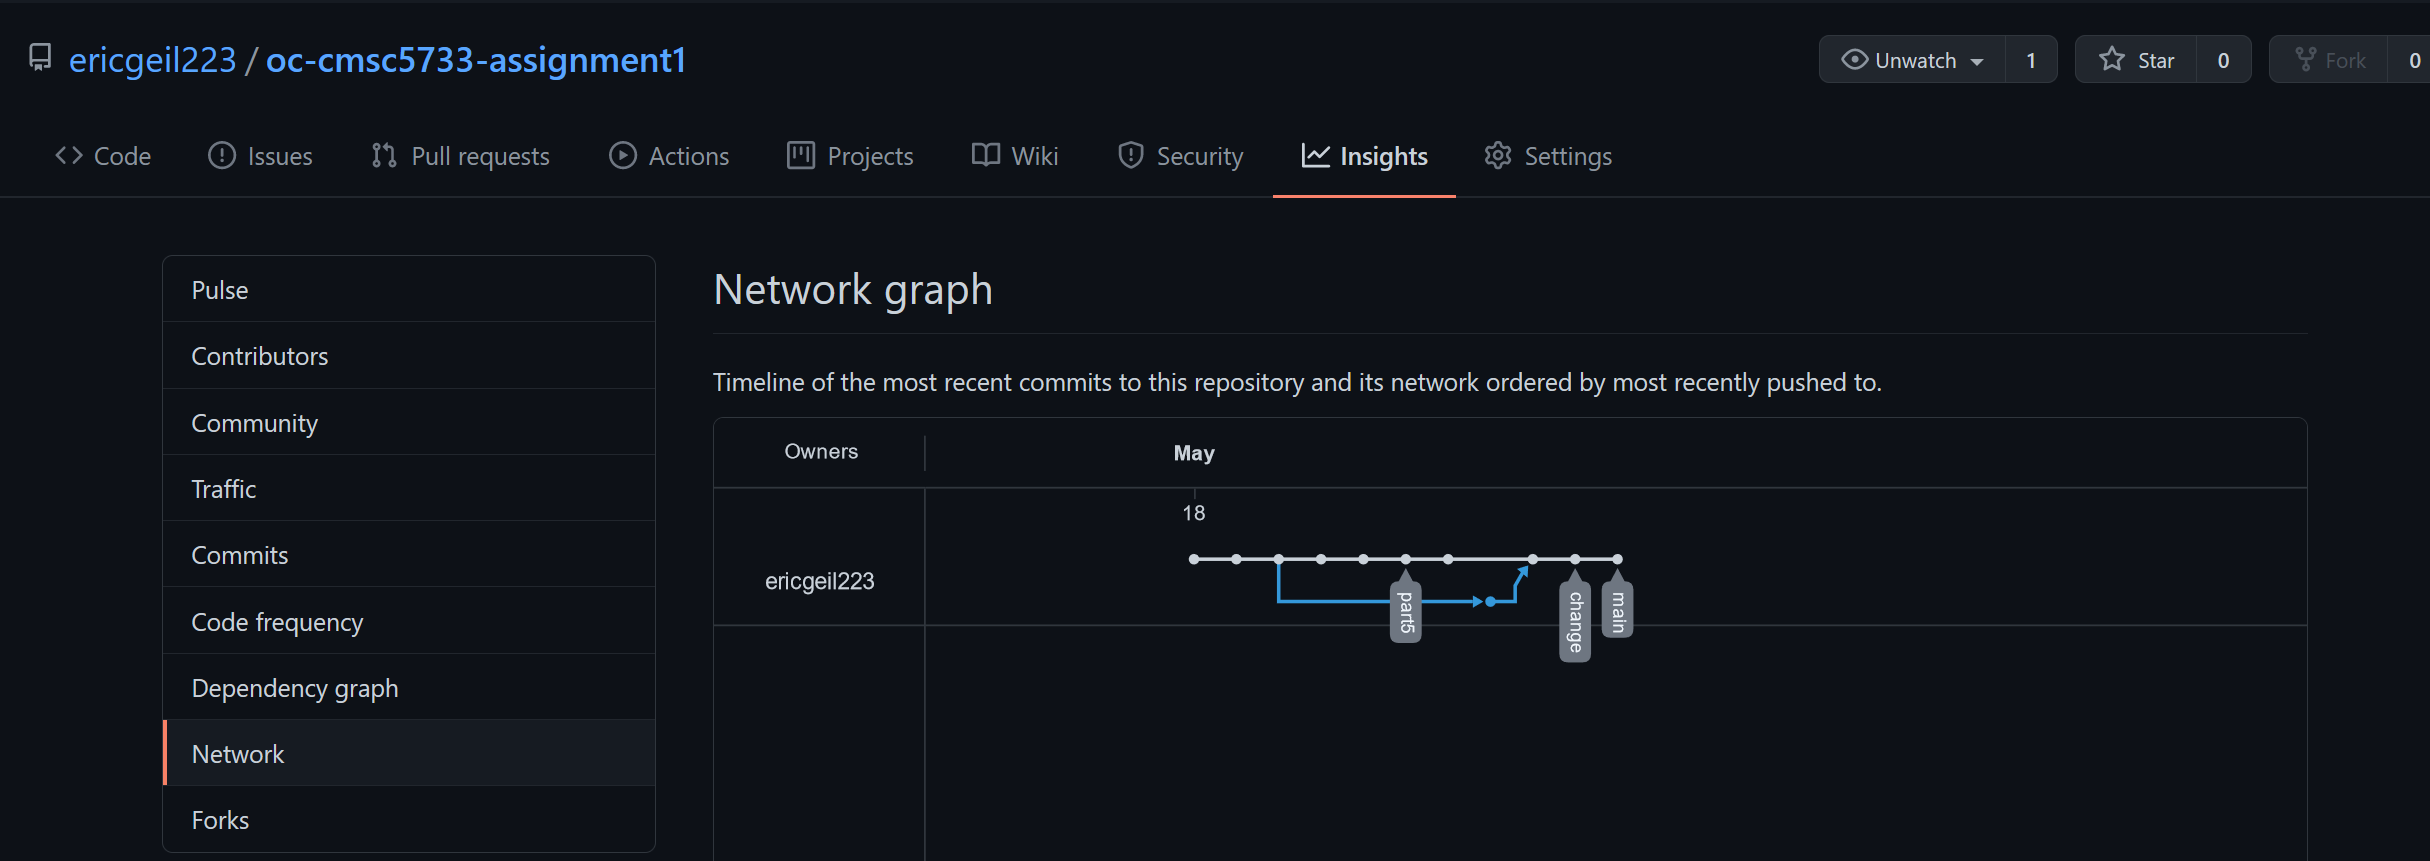
\includegraphics[width=1.0\textwidth]{4.png}
\end{document}